\documentclass{article}
\usepackage{amsmath}
\usepackage{graphicx}
\usepackage{lettrine}

\begin{document}


\begin{titlepage}
    \centering
    \vspace*{1cm}
    
    \Huge
    \textbf{Planes and Birds: Minimizing energy}
    
    \vspace{0.5cm}
    
    \Large
    Tao Su
    \vspace{1.5cm}

    \large 
    \textit{HornorsCalc1 Fall 2024 Project Final}
    \vfill

    \begin{figure}[h]
        \centering
        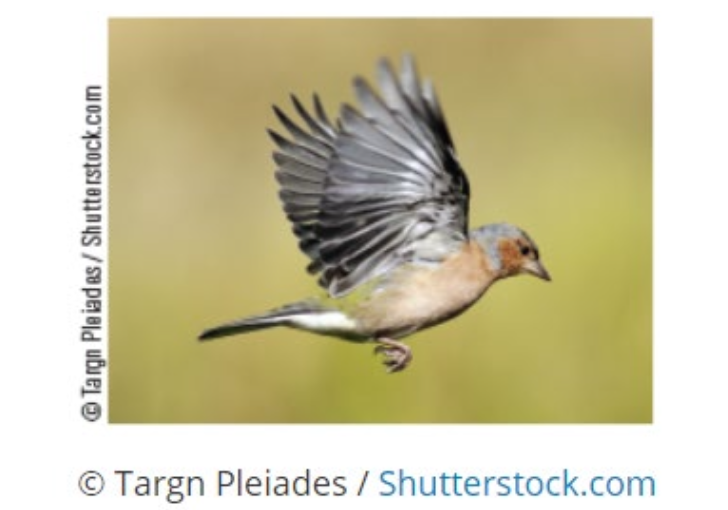
\includegraphics[width=1\textwidth]{coverPage.png}
        \caption{\small A flying Bird}
        \label{fig:cover}
    \end{figure}
            
    \Large
    \today  % or you can replace with a specific date
    
\end{titlepage}

\newpage

\subsection*{The Introduction}

\lettrine[lines=2]{S}{mall} birds, such as finches, alternate between flapping their wings and gliding, a behavior that is essential to their flight dynamics and energy conservation.

In this project, I will focus on understanding how the speed of a bird affects the lift power and the average energy spent during flight.

By using derivatives, the aim of this project is to examine the relationship between flight speed, lift power, and energy expenditure.

While the principles involved are similar to those of fixed-wing aircraft, my primary objective is to apply mathematical analysis to explore how changes in speed influence the energy efficiency of flight.

Through this approach, we seek to gain a deeper understanding of the forces at play and the optimal conditions for minimizing energy expenditure in birds during flight.


\subsection*{Part 1:}
\begin{figure}[h]
    \centering
    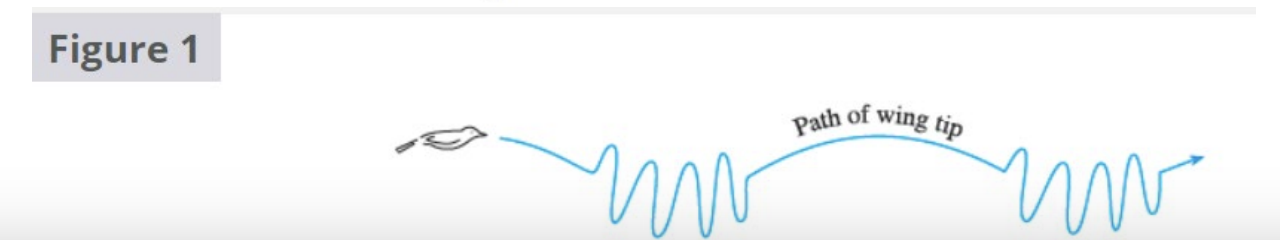
\includegraphics[width=0.5\textwidth]{bird.png}
    \caption{\small The trajectory of a flying bird.}
    \label{fig:bird}
\end{figure}

The power needed to propel an airplane forward at velocity \( v \) is: 
\[
P = Av^3 + \frac{BL^2}{v}.
\]
where \( A \) and \( B \) are positive constants specific to the particular aircraft, and \( L \) is the lift—the upward force supporting the weight of the plane (or bird).
\setlength{\parskip}{2em}

To determine the relationship between the power \(P\) and the speed \(v\), we can start with finding the derivative of \(P'\) with respect to \(v\).

The derivative of \( P \) with respect to \( v \) is:
\[
P'(v) = 3Av^2 - \frac{BL^2}{v^2}.
\]

To find the critical point of \( P(v) \), we set \( P'(v) = 0 \):
\[
P'(v) = 3Av^2 - \frac{BL^2}{v^2} = 0.
\]
Solving for \( v \), we get:
\[
v^4 = \frac{BL^2}{3A}.
\]
Therefore, we can find the speed \( V \) as:
\[
V = \sqrt[4]{\frac{BL^2}{3A}}.
\]

To determine whether this speed represents a minimum or maximum, we test the second derivative:
\[
P''(v) = 6Av + \frac{2BL^2}{v^3}.
\]

Since \( A \) and \( B \) are positive constants, and \( L^2 \) and \( v \) are always positive, we find that:
\[
P''(v) = 6Av + \frac{2BL^2}{v^3} > 0.
\]

Thus, when \( P'(v) = 0 \) and \( P''(v) > 0 \), \( P \) concaved up, indicating an absolute minimum. Therefore, when
\[
V = \sqrt[4]{\frac{BL^2}{3A}},
\]
the required power \( P \) is minimized.

\subsection*{Part 2:}
The speed found in Part 1 minimizes power, but a faster speed might use less fuel. The energy needed to propel the airplane/bird a unit distance is \( E = \frac{P}{v} \). At what speed is energy minimized?

To find out the answer, we first need to know the relationship between \( E \) and \( v \). 

Fortunately, we know:
\[
P = Av^3 + \frac{BL^2}{v} \text{ from the beginning, and }
E = \frac{P}{v}
\]

So, we can easily derive the equation for \( E(v) \):
\[
E = Av^2 + \frac{BL^2}{v^2}
\]
Next, let's take the derivative of \(E\) respect to \(v\):
\[
E'(v) = 2Av-\frac{2BL^2}{v^3}
\]
Same as part 1, we also need to find the critical point of \(E'(v)\):
\[\text{We set } E'(v) = 2Av-\frac{2BL^2}{v^3} = 0,\text{ solve for }v, v^4=\frac{2BL^2}{2A}, v = \sqrt[4]{\frac{BL^2}{A}}\text{.}\]
Then we take the second derivative of \(E'\) respect to \(v\):
\[E''(v) = 2A + \frac{6BL^2}{v^4},
\text{ because } 2A > 0, \text{ and } \frac{6BL^2}{v^4} > 0, E''(v) > 0.\]
Therefore,
 \[\text{when the speed }v = \sqrt[4]{\frac{BL^2}{A}}, E\text{ has the absolute minimum,}\]
  the energy is minimized.

\subsection*{Part 3:}
How much faster is the speed for minimum energy than the speed for minimum power?

\end{document}